\PassOptionsToPackage{ukrainian,english}{babel}
\documentclass[twocolumn]{el-author}

%\usepackage[...]{...}      This has been commented out as we are not using any additional packages here.  On the whole, they should be unnecessary.
\usepackage{mathtext}
\usepackage[T1,T2A]{fontenc}
\usepackage[english,ukrainian]{babel}
\usepackage{hyperref}
\usepackage{graphicx} %package to manage images
\usepackage[a4paper, total={7in, 9.5in}]{geometry}
\usepackage{makecell}
\graphicspath{ {images/} }
\newcommand{\hH}{\hat{H}}
\newcommand{\D}{^\dagger}
\newcommand{\ua}{\uparrow}
\newcommand{\nc}{\newcommand}
\renewcommand\theadfont{\normalsize\scshape}
\nc{\da}{\downarrow} \nc{\hc}{\hat{c}} \nc{\hS}{\hat{S}}
\nc{\bra}{\langle} \nc{\ket}{\rangle} \nc{\eq}{equation (\ref}
\nc{\h}{\hat} \nc{\hT}{\h{T}}\nc{\be}{\begin{eqnarray}}
\nc{\ee}{\end{eqnarray}}\nc{\rd}{\textrm{d}}\nc{\e}{eqnarray}\nc{\hR}{\hat{R}}\nc{\Tr}{\mathrm{Tr}}
\nc{\tS}{\tilde{S}}\nc{\tr}{\mathrm{tr}}\nc{\8}{\infty}\nc{\lgs}{\bra\ua,\phi|}\nc{\rgs}{|\ua,\phi\ket}
\nc{\hU}{\hat{U}}\nc{\lfs}{\bra\phi|}\nc{\rfs}{|\phi\ket}\nc{\hZ}{\hat{Z}}\nc{\hd}{\hat{d}}\nc{\mD}{\mathcal{D}}
\nc{\bd}{\bar{d}}\nc{\bc}{\bar{c}}\nc{\mc}{\mathcal}\nc{\ea}{eqnarray}\nc{\mG}{\mathcal{G}}\nc{\bce}{\begin{center}}
\nc{\ece}{\end{center}}
\date{20 Грудня 2018}

\begin{document}

\title{Визначення сталої Стефана - Больцмана}

\author{Сергій Поліщук}

\abstract{Стала Стефана — Больцмана визначає зв'язок між потоком випромінювання й ефективною температурою тіла, що випромінює як абсолютно чорне тіло.}

\maketitle

\section{Мета роботи}

вивчити закони теплового випромінювання. 

\section{Прилади і матеріали}

пірометр з телескопом ТЕРА-50, електрична
лампочка, ЛАТР, вольтметр, амперметр, лінійка.

\section{Завдання}

\begin{enumerate}
	\item при домашній підготовці:
	\begin{itemize}
		\item  користуючись рекомендованою літературою, вивчити
			закономірності теплового випромінювання;
		\item  3 фізичного практикуму записати теоретичні відомості,
			порядок виконання роботи, зарисувати оптичну та електричну
			схеми;
		\item  вивчити будову та принцип дії пірометра.
	\end{itemize}
	\item при виконанні роботи:
	\begin{itemize}
		\item  скласти електричну схему і показати її викладачеві для
			перевірки;
		\item  визначити температуру спіралі в лампи розжарювання
			безконтактним методом за її тепловим випромінюванням;
		\item  визначити сталу у законі Стефана - Больцмана;
		\item  виконати необхідні розрахунки з визначення шуканої
			величини та можливих похибок;
		\item  оформити звіт і подати його викладачеві.
	\end{itemize}
	
\end{enumerate}

\section{Правила техніки безпеки}

\begin{itemize}
	\item  бережіться пошкодження очей при роботі з ТЕРА-50;
	\item  при складанні електричної схеми використовуйте провідники
		з непошкодженою ізоляцією;
	\item  прикористуванні ЛАТРОм будьте уважні - напруга 220В!
\end{itemize}

\section{Теоретичні відомості та опис установки}

У становленні квантової механіки значну роль відіграло вивчення
закономірностей теплового випромінювання, а в ньому -- введення Г. Кірхго-
фом (1862р.) абстракції абсолютно чорного тіла. Це таке ідеалізоване тіло, яке
поглинає все падаюче на нього випромінювання будь-яких частот при будь-
яких температурах, поглинаюча здатність для нього рівна одиниці. Кірхгофом
також було встановлено, що випромінювальна здатність тіл, температури яких
однакові, найбільша саме у абсолютно чорного. Ця обставина зумовила у
подальшому пошук тих параметрів, від яких залежить випромінювання чорного
тіла, та їх взаємозв'язку. Перший крок у цьому напрямку був зроблений
Й. Стефаном (1879 р.), який, на основі виконаних ним та іншими дослідниками
експрементальних вимірювань, висловив здогадку, що повна енергія,
випромінювана з одиниці поверхні тіла за одиницю часу, залежить лише від
температури і пропорційна четвертому степеню абсолютної температури тіла.
Пізніше (1884 р.) Л. Больцман теоретичними розрахунками підтвердив не
припущення. Таким чином, було встановлено, що повна (інтегральна)
випромінювальна здатність абсолютно чорного тіла Е є функцією лише
температури Т і пропорційна четвертому степеню цієї температури. Тобто

\begin{equation} \label{eq:Stefan_Boltzmann}
E(T) = \sigma T^{4}
\end{equation}

Цей вираз одержав назву закону Стефана - Больцмана, а коефіцієнт $\sigma$
- сталої Стефана - Больцмана. Ретельні вимірювання показали, що

\begin{equation} \label{eq:Stefan_Boltzmann_const}
\sigma = 5.67 \cdot 10^{-8} Вт.(м^{2} \cdot K^{4})
\end{equation}

Одним із завдань даної роботи є експериментальне визначення сталої $\sigma$.

\begin{figure}[ht]
\centering{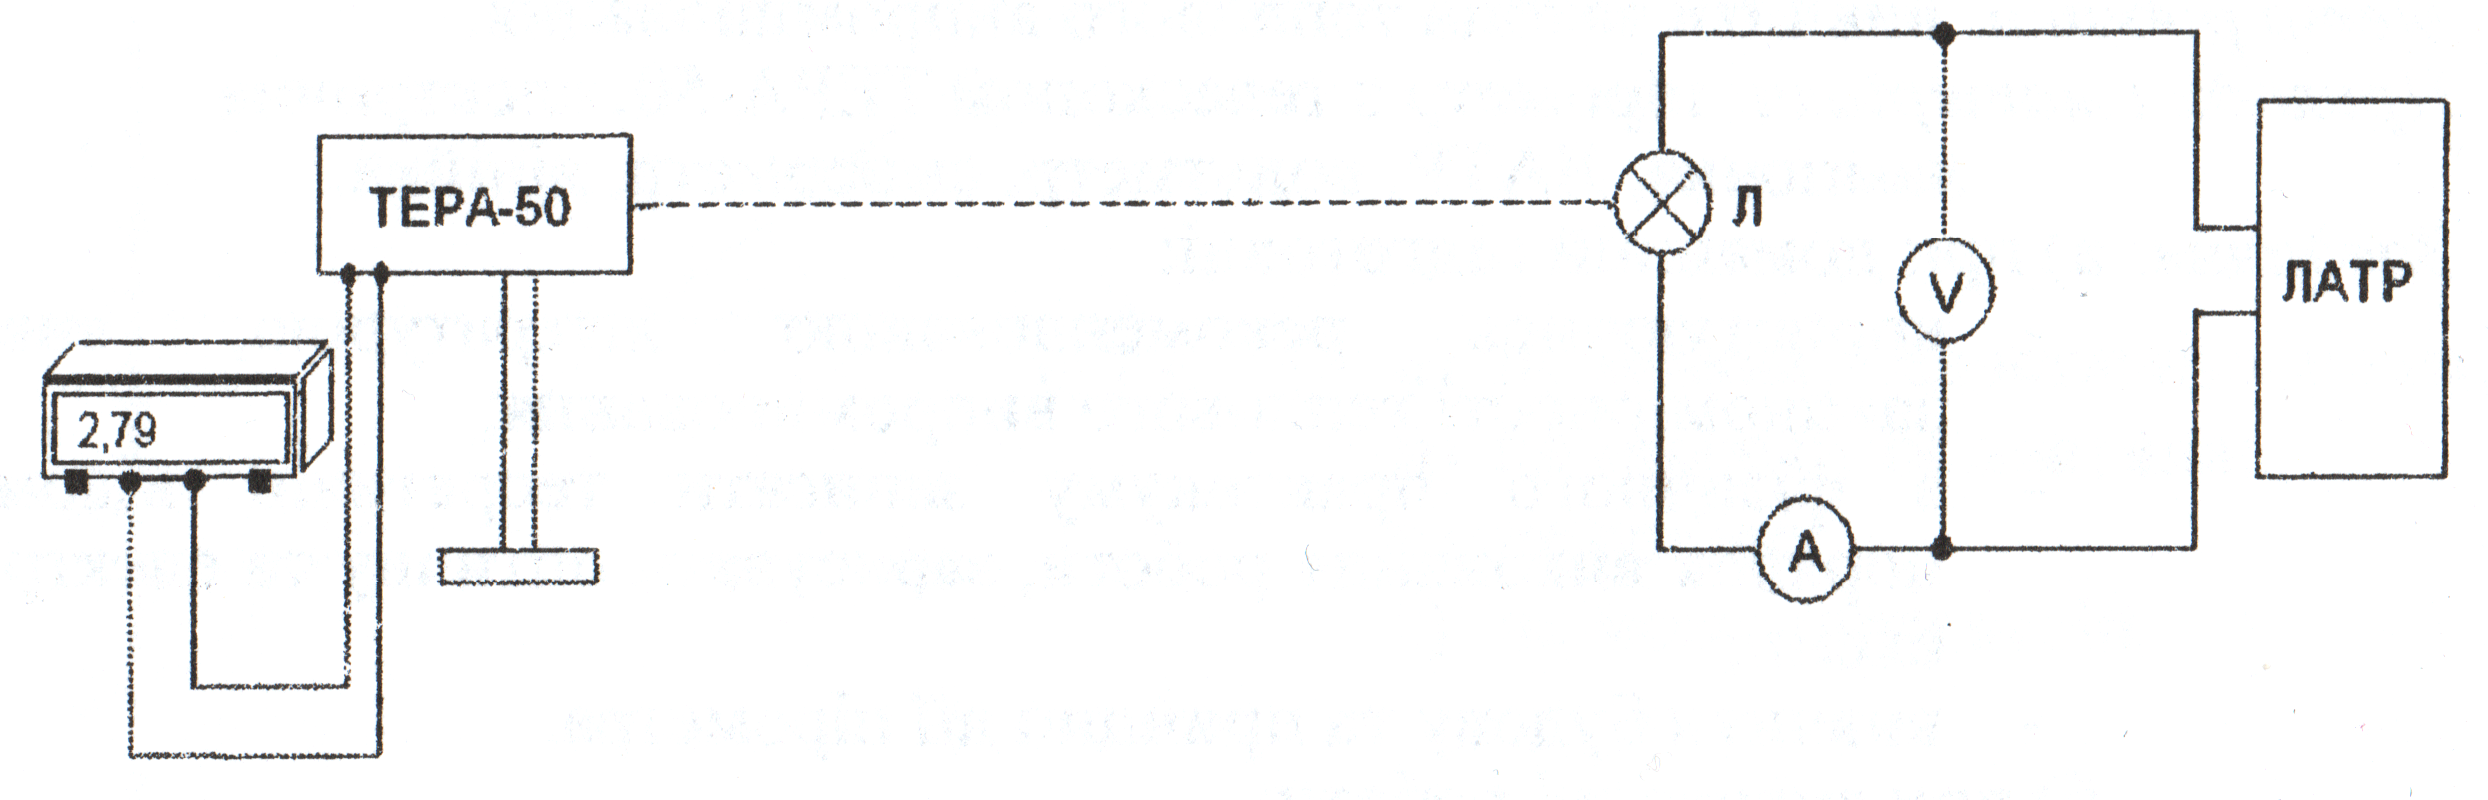
\includegraphics[width=80mm]{img_1}}
\caption{\source{}}
\label{img:1}
\end{figure}

З цією метою зібрана установка (рис.\ref{img:1}), яка складається з кола джерела
випромінювання та кола приймача випромінювання. Як випромінювач
застосовується лампа розжарення з широкою плоскою спіраллю. Регульована
напруга на неї подається від  автотрансформатора.  Приймачем
випромінювання слугує пірометр з телескопом ТЕРА-50. Припускається, що
потужність електричного струму, яким живиться лампа, пропорційна
потужності випромінювання з поверхні її спіралі. 
Тобто $\frac{IU}{S} ~ \sigma T^{4}$ 
де $S$ - площа видимої у телескоп ТЕРА-50 розжареної спіралі лампи.

Якщо дослідження відбуваються у середовищі з температурою $T_{0}$
(у нашому випадку це абсолютна температура повітря у лабораторії), то
$\frac{IU}{S} ~ \sigma(T^{4} - T_{0}^{4})$ або 
$IU = a_{r}S (T^{4} - T_{0}^{4}) \cdot \sigma$. Звідки

\begin{equation} \label{eq:1}
\sigma = \frac{IU}{a_{r}S(T^{4} - T_{0}^{4})}
\end{equation}

Коефіцієнт $a_{r}$ - це стала приладу, яка залежить від ряду обставин, зокрема,
враховує те, що спіраль лампи не є абсолютно чорним тілом, що не вся
електрична енергія перетворюється у випромінювання тощо.

Крім того, а, залежить і від температури випромінювача. Значення $a_{r} \cdot S$
для деяких температур наведені у таблиці~\ref{tab:1}. Тут же подано співвідношення
між напругою на виході пірометра та температурою випромінювача.

Таблиця складена для випадку, коли відстань між джерелом
випромінювання і приймачем становить 1 м.

\begin{table}[ht]
\caption{\label{tab:1} }
{\begin{tabular}{|l|l|l|}\hline
\thead{Напруга на виході \\ пірометра, мВ} & 
\thead{Температура \\ випромінювача, $ _{0} C$} & 
\thead{Значення $a_{r} \cdot S $, $м^{2}$} \\\hline
0.41 & 500 & $2.5*10^{-3}$ \\\hline
0.82 & 600 & $2.7*10^{-3}$ \\\hline
1.56 & 700 & $2.9*10^{-3}$ \\\hline
2.79 & 800 & $3.3*10^{-3}$ \\\hline
4.58 & 900 & $3.5*10^{-3}$ \\\hline
7.05 & 1000 & $3.8*10^{-3}$ \\\hline
\end{tabular}}{}
\end{table}

\newpage

\section{Послідовність виконання роботи}

\begin{enumerate}
	\item Скласти електричну схему згідно рис.2.1, показати її для перевірки
		викладачеві.
	\item Автотрансформатором встановити таку напругу на лампі, щоб її
		спіраль ледь жевріла.
	\item Телескоп  ТЕРА-50 встановити на відстані Ім від лампи |і
		відрегулювати його таким чином, щоб спіраль лампи потрапила у
		центр поля зору телескопа. Площина спіралі при цьому повинна а бути
		паралельна об'єктиву телескопа.
	\item Поступово збільшуючи автотрансформатором напругу на лампі,
		домогтися, щоб напруга на виході пірометра становила 0,41 мВ, що
		відповідає температурі спіралі лампи 500$^{0}C$.
	\item Зняти покази вольтметра та амперметра і за формулою~(\ref{eq:1}) 	
		визначити сталу $\sigma$.
	\item Подібним чином визначити сталу Стефана -- Больцмана для решти
		температур, що вказані у таблиці~\ref{tab:1}.
	\item Виконати математичну обробку одержаних результатів, провести їх
		аналіз і порівняти експериментально юдержане значення $\sigma$ з
		табличним.
\end{enumerate}

\begin{thebibliography}{}

\bibitem{1}
Кучерук І.М., Горбачук ІТ. Загальний курс фізики: Т.3.: Оптика.
Квантова фізика. -- К.: Техніка, 2006. -- 518с., ст. 260 - 266.

\bibitem{2}
Кучерук І.М, Дущенко В.П. Загальна фізика. Оптика. Квантова
фізика. - К.: Вища школа, 1991. -- 463с., ст. 281 - 291.

\bibitem{3}
 Горбачук І.Т. Загальна фізика. Лабораторний практикум. - К.:
Вища школа, 1992.- 512 с., ст. 424 - 429

\bibitem{4}
Дущенко В.П. Фізичний практикум. - К. Вища школа, 1984. --
256с., ст. 185 - 191.

\bibitem{5}
Методична розробка до роботи.

\end{thebibliography}

\section{Завдання для самоконтролю}

\begin{enumerate}
	\item Що таке теплове випромінювання?
	\item Які особливості теплового випромінювання?
	\item У чому полягає закон Стефана -- Больцмана?
	\item Які тіла можна вважати абсолютно чорними?
	\item Який вигляд має закон Стефана - Больцмана для сірих тіл?
	\item Що таке повна випромінювальна здатність тіла?
	\item Який вигляд має крива розподілу енергії в спектрі чорного
випромінювання?
	\item Який фізичний зміст площі, обмеженої кривою розподілу енергії
в спектрі чорного випромінювання?
	\item Наведіть приклади моделей абсолютно чорного тіла.
	\item Яка будова та принцип дії телескопа ТЕРА-50?
\end{enumerate}

\newpage
\section{Тестові завдання для вхідного контролю}

\begin{enumerate}
	\item Характерною ознакою теплового випромінювання є його:
	\begin{enumerate}
		\item хаотичність;
		\item ізотропність;
		\item рівноважність;
		\item неполяризованість.
	\end{enumerate}
	\item Яка з перелічених нижче здатностей не притаманна тепловому
випромінюванню?
	\begin{enumerate}
		\item випромінювальна;
		\item поглинальна;
		\item розсіювальна;
		\item відбивна.
	\end{enumerate}
	\item Для абсолютно чорного тіла дорівнює нулеві:
	\begin{enumerate}
		\item поглинальна здатність;
		\item поглинальна і відбивна здатність;
		\item відбивна і пропускна здатність;
		\item пропускна і поглинальна здатність.
	\end{enumerate}
	\item Зв'язок між температурною шкалою Цельсія і температурною шкалою
Кельвіна має вигляд:
	\begin{enumerate}
		\item $t^{0}C = 273 - TK$;
		\item $t^{0}C = TK - 273$;
		\item $t^{0}C = 273 + TK$;
		\item $t^{0}C = -TK -273$.
	\end{enumerate}
	\item Характер випромінювання абсолютно чорного тіла залежить від:
	\begin{enumerate}
		\item природи тіла;
		\item стану поверхні тіла;
		\item температури;
		\item агрегатного стану.
	\end{enumerate}
	\item Яке співвідношення між випромінювальними здатностями реального і
абсолютно чорного тіла? Тіла мають однакову температуру.
	\begin{enumerate}
		\item випромінювальні здатності однакові;
		\item випромінювальна здатність більша у абсолютно чорного тіла;
		\item реальне тіло має більшу випромінювальну здатність;
		\item співвідношення може бути будь-яким.
	\end{enumerate}
	\item Зв'язок між спектральною випромінювальною здатністю тіла $E(v, T)$ і Його
повною випромінювальною здатністю $E(T)$ має вигляд:
	\begin{enumerate}
		\item $E(v,T) = \int_{0}^{\infty}E(T)dv$;
		\item $E(T) =   \int_{0}^{\infty}\frac{E(v,T)}{dv}$;
		\item $E(v,T) = E(T)$;
		\item $E(T) =   \int_{0}^{\infty}E(v,T)dv$.
	\end{enumerate}
	\item Закон Стефана-Больцмана для абсолютно чорного тіла має вигляд:
	\begin{enumerate}
		\item $E(T) = \sigma T^{3}$;
		\item $E(T) = \sigma T^{4}$;
		\item $E(T) = \sigma ^{4} T$;
		\item $E(T) = (\sigma T)^{4}$.
	\end{enumerate}
	\item Стала Стефана -- Больцмана $\sigma$ має значення:
	\begin{enumerate}
		\item $5.67 \cdot 10^{-8}$;
		\item $2.89 \cdot 10^{-3}$;
		\item $1.38 \cdot 10^{-23}$;
		\item $8.31 \cdot 10^{3}$.
	\end{enumerate}
	\newpage
	\item Стала Стефана-Больцмана у цій роботі визначається виразом:
	\begin{enumerate}
		\item $\sigma = \frac{a_{r} \cdot S(T^{4} - T_{0}^{4})}{IU}$;
		\item $\sigma = \frac{a_{r} \cdot S \cdot I \cdot U}{(T^{4} - T_{0}^{4})}$;
		\item $\sigma = \frac{(T^{4} - T_{0}^{4})}{a_{r} \cdot S \cdot I \cdot U}$;
		\item $\sigma = \frac{I \cdot U}{a_{r} \cdot S(T^{4} -  T_{0}^{4})}$.
	\end{enumerate}
\end{enumerate}

\section{Тестові завдання для підсумкового контролю}

\begin{enumerate}
	\item Яке з нижче наведення співвідношень між повною випромінювальною
здатністю $E(T)$, спектральною випромінювальною здатністю $E(v, T)$,
поглинальною здатністю $a(v,T)$, відбивною здатністю $r(v, T)$, пропускною
здатністю $D(v,T)$ тіла є вірними?
	\begin{enumerate}
		\item $E(v,T) + a(v,T) + r(v,T) = 1$;
		\item $r(v,T) + a(v,T) + D(v,T) = 1$;
		\item $E(T) + D(v,T) + a(v,T) = 1$;
		\item $E(v,T) + r(v,T) + D(v,T) = 1$.
	\end{enumerate}
	\item Закон Кірхгофа для теплового випромінювання має вигляд:
	\begin{enumerate}
		\item $\frac{E(v,T)}{\varepsilon (v,T)} = a(v,T)$;
		\item $\frac{a(v,T)}{E(v,T)} = \varepsilon (v,T)$;
		\item $\frac{\varepsilon (v,T)}{a(v,T)} = E(v,T)$;
		\item $\frac{E(v,T)}{a(v,T} = \varepsilon (v,T)$.
	\end{enumerate}
	де $E(v,T)$ і $a(v,T)$ - спектральні випромінювальна і поглинальна здатності тіла,
	$\varepsilon (v,T)$ - спектральна випромінювальна здатність абсолютно чорного тіла.
	\item ід яких з нижче перелічених чинників залежить випромінювальна
здатність реальних тіл: 1) температури, 2) хімічного складу, 3) фізичного
стану, 4) чистоти поверхні?
	\begin{enumerate}
		\item лише від першого;
		\item від першого і другого;
		\item лише від третього;
		\item від усіх чотирьох.
	\end{enumerate}
	\item При кімнатній температурі шматок кераміки має зелений колір. Який буде
його колір у розжареному стані?
	\begin{enumerate}
		\item зелений;
		\item жовтогарячий;
		\item лілово-фіолетовий;
		\item червоно-оранжевий.
	\end{enumerate}
	\item Закон зміщення Віна має вигляд:
	\begin{enumerate}
		\item $\lambda _{max} \cdot T = b$;
		\item $\lambda _{max} \cdot T^{2} = b$;
		\item $\lambda _{max} \cdot T^{3} = b$;
		\item $\lambda _{max} \cdot T^{4} = b$.
	\end{enumerate}
	\item Константа у законі зміщення Віна рівна:
	\begin{enumerate}
		\item $5.67 \cdot 10^{-8}$;
		\item $2.9 \cdot 10^{-3}$;
		\item $1.38 \cdot 10^{-23}$;
		\item $8.31 \cdot 10^{3}$.
	\end{enumerate}
	\item У законі зміщення Віна $v_{max}$ це:
	\begin{enumerate}
		\item максимальна частота, яку може випромінювати абсолютно чорне тіло;
		\item максимальна частота, яку випромінює нагріте до температури 7 тіло;
		\item частота, яка відповідає максимуму випромінювальної здатності тіла;
		\item частота, яка відповідає короткохвильовій межі випромінювання.
	\end{enumerate}
	\item Формула Релея-Джинса для спектральної випромінювальної здатності
		абсолютно чорного тіла має вигляд:
	\begin{enumerate}
		\item $\varepsilon (v,T) = \frac{kT}{2 \pi} (\frac{v}{c})^{2}$;
		\item $\varepsilon (v,T) = \frac{2 \pi}{kT} (\frac{c}{v})^{2}$;
		\item $\varepsilon (v,T) = (2 \pi \frac{v}{c})^{2}$;
		\item $\varepsilon (v,T) = (\frac{2 \pi v ^{2}}{c^{2}}) \cdot kT$;
	\end{enumerate}
	\item Формула Планка для випромінювальної здатності абсолютно чорного тіла:
	\begin{enumerate}
		\item $\varepsilon (v,T) = 2 \pi (\frac{v}{c})^{2} \cdot \frac{hv}{exp(\frac{hv}{kT}) -1}$;
		\item $\varepsilon (v,T) = (2 \pi \frac{v}{c})^{2} \cdot \frac{kT}{exp(\frac{kT}{hv}) - 1}$;
		\item $\varepsilon (v,T) = \frac{hv}{2 \pi}(\frac{v}{c})^{2} \cdot \frac{1}{exp(\frac{hv}{kT}) - 1}$;
		\item $\varepsilon (v,T) = (\frac{c}{v})^{2} \cdot \frac{2 \pi}{exp(\frac{kT}{hv}) - 1}$.
	\end{enumerate}
	\item Реальні фізичні тіла, які існують у природі, можна вважати:
	\begin{enumerate}
		\item чорними;
		\item сірими;
		\item білими;
		\item селективними.
	\end{enumerate}
\end{enumerate}

\end{document}

%\begin{table}[b]
%\processtable{Coefficients and remainders for distribution KK ($k = 0.05$,
%$v = 3$, $c_{1} = 1.5$, $c_{2} = 4.5$)}
%{\begin{tabular}{|l|l|l|}\hline
%$n$ & $a_{n}^{2}$ & $r_{k}(1)$\\\hline
%0 & 3.602576748428 & 1.493719547999\\\hline
%1 & 1.384791111989 & 0.108928436101\\\hline
%2 & 0.108600438794 & 0.000327997399\\\hline
%3 & 0.000275794597 & 0.000052202814\\\hline
%4 & 0.000027616892 & 0.000024585922\\\hline
%5 & 0.000018178621 & 0.000006407300\\\hline
%\end{tabular}}{}
%\end{table}
%
%So, the basic preamble and main body will be:
%\verb"\documentclass[twocolumn]{el-author}"\\
%\verb"\usepackage[...]{packages}"\\
%\verb"\date{12 December 2012}"\\
%\verb"\title{...}"\\
%\verb"\author{...}"\\
%\verb"\abstract{...}"\\
%\verb"\maketitle{...}"\\
%\verb"\begin{document}"\\
%\verb"..."\\
%\verb"\section{...}"\\
%\verb"..."\\
%\verb"\section{..}"\\
%\verb"..."\\
%\verb"\end{document}"